\documentclass[10pt, twocolumn]{article}

% --- Packages ---
\usepackage[utf8]{inputenc}    % Standard encoding
\usepackage[margin=0.75in]{geometry} % Page margins
\usepackage{graphicx}          % For including images
\usepackage{amsmath, amssymb}  % Essential math symbols
\usepackage{booktabs}          % Professional quality tables
\usepackage[backend=biber, style=ieee]{biblatex}
\addbibresource{references.bib}
\setlength{\abovecaptionskip}{-2pt}

% --- Title Information ---
\title{\textbf{Project 1: Imaging Fundamentals}}
\author{Sophia Klymchuk \\ \textit{ECE-435: Medical Imaging}}
\date{February 25, 2026}
\begin{document}

\maketitle

\begin{abstract}
This project explores the fundamental principles of medical image reconstruction and processing using a thoracic CT dataset. Methods explored include slicing, various types of filtering for noise reduction, and edge detection techniques.
\end{abstract} 

\section{Introduction}
Medical imaging relies on the accurate transformation of raw acquisition data into interpretable representations. This process requires a precise understanding of coordinate mapping, voxel isotropy, and the noise characteristics inherent in digital systems. In Computed Tomography (CT), image quality is often degraded by stochastic noise and system-induced blur, necessitating robust digital processing techniques to preserve diagnostic utility.

\section{Methodology}
The original dataset \cite{Mulrecon} consists of 237 two-dimensional JPEG images representing an image slice through the thorax at fixed intervals along the $z$-axis. The given DICOM attributes are (Pixel Spacing 0.703 mm 0028,0030; Slice Thickness 1.25 mm 0018,0050; Spacing Between Slides 0.625 mm 0018,0088; Number of slices 237), where the pixel spacing defines the physical distance between adjacent pixels in the $x$ and $y$ directions \cite{PixelSpacingAttribute}, while the slice thickness and spacing between slides define the distance between adjacent slices along the $z$-axis \cite{SliceThicknessAttribute}. The images are 8-bit grayscale with dimensions of $512 \times 512$ pixels, and the pixel intensity values range from $0$ (black) to $255$ (white). The dataset is organized in a directory structure where each image file is named sequentially (e.g., "axial00001.jpg", "axial00002.jpg", ..., "axial00237.jpg"), corresponding to their position along the $z$-axis. 

\subsection{Slicing}

 To transition from a sequence of 2D images to a functional 3D volume, a right-handed Cartesian coordinate system was established. The stack was mapped into a 3D grayscale array, $V$, where the first index corresponds to the $x$ pixel, the second to the $y$ pixel, and the third to the $z$ pixel (image index). The relationship between the array indices, anatomical axes, and the resulting planes is summarized in Table \ref{tab:integrated_mapping} \cite{AnatomicalTerminologySEER}.

\begin{table*}[t]
\centering
\caption{Integrated Mapping of Anatomical Planes, Cartesian Axes, and Array Slicing}
\label{tab:integrated_mapping}
\begin{tabular}{@{}lllll@{}}
\toprule
\textbf{Anatomical Plane} & \textbf{Fixed Axis} & \textbf{Anatomical Directions} & \textbf{Cartesian} & \textbf{Slice Index} \\ \midrule
Axial (Transverse)        & $z$ (Longitudinal)  & inferior $\to$ superior        & $-z, +z$           & $V(:,:,p)$           \\
Coronal (Frontal)         & $y$ (Anteroposterior)& posterior $\to$ anterior       & $-y, +y$           & $V(:,p,:)$           \\
Sagittal (Longitudinal)   & $x$ (Mediolateral)  & left $\to$ right               & $-x, +x$           & $V(p,:,:)$           \\ \bottomrule
\end{tabular}
\end{table*}

The reconstruction followed a three-step transformation to ensure the volume adhered to a standard right-handed Cartesian coordinate system ($x, y, z$). Firstly, the images were read sequentially and stacked along a new third axis using \texttt{numpy.stack}. This initially produced an array with the shape $(z, y, x)$. Then, to meet the requirement that the first, second, and third indices correspond to the $x$, $y$, and $z$ pixels respectively, the array was transposed from $(z, y, x)$ to $(x, y, z)$. Finally, because standard image indexing (top-down) often conflicts with Cartesian coordinates (bottom-up), the $y$-axis was flipped. This ensures that "up" in the anatomical image corresponds to an increasing $y$ value, correcting the "upside down" orientation when rendered with a lower origin.

The resulting volume is anisotropic, meaning the physical dimensions of a voxel (a 3D pixel) are not equal in all directions. The spatial resolution of the scan is defined by two parameters, as given by the dataset's DICOM parameters \cite{Mulrecon}. The axial plane resolution (pixel spacing) is $0.703$ mm/pixel along the $x$ and $y$ axes. The resolution along the $z$ axis (slice spacing) is $0.625$ mm/slice. To prevent anatomical distortion during the visualization of the Coronal ($xz$) and Sagittal ($yz$) planes, a scaling factor, $z_{aspect}$, was applied: 
$$z_{aspect} = \frac{\text{Slice Spacing}}{\text{Pixel Spacing}} = \frac{0.625\text{ mm}}{0.703\text{ mm}} \approx 0.889$$
This ratio is used during rendering to adjust the display height of the $z$-axis, ensuring that a pixel in $x$ represents the same physical distance as a pixel in $z$.

\subsection{Salt and Pepper}
Salt-and-pepper noise (SPN) is common in CT images and typically results from acquisition or digitization errors \cite{alrabaieMultipleNoisesRemoval2018}. It appears as random pixels with extreme intensities. If $z$ is a pixel intensity, its probability density function is:
\begin{equation}
p(z) = 
\begin{cases} 
p_{salt} & \text{for } z = a \\
p_{pepper} & \text{for } z = b \\
0 & \text{otherwise}
\end{cases}
\end{equation}

In 8-bit images, $a = 255$ (salt) and $b = 0$ (pepper), while the original intensity is retained with probability $1 - p_{salt} - p_{pepper}$.

Mean and median filters are commonly used for noise reduction. The mean filter is a linear low-pass filter that replaces each pixel with the average of its $m \times n$ neighborhood. Because it averages values, it is sensitive to outliers; even a single salt or pepper pixel in a small window can significantly distort the result and spread the artifact.

The median filter is nonlinear and replaces the center pixel with the median intensity in the neighborhood. Since SPN produces extreme values, these outliers move to the ends of the ordered sequence, allowing the median to select a likely uncorrupted value. This removes noise more effectively while preserving edges.

To evaluate performance, mean and median filters were applied to the uncorrupted axial slice displayed in Figure \ref{fig:axial_slice}, using $3 \times 3$ and $5 \times 5$ kernels. We utilized the functions \texttt{cv2.blur} and \texttt{cv2.medianBlur} for mean and median filtering, respectively. Noise robustness was then tested by adding synthetic SPN to the image: each pixel was randomly assigned salt with probability $p$, pepper with probability $p$, or left unchanged with probability $1 - 2p$. Three noisy images were generated with $p \in \{0.01, 0.05, 0.10\}$, and each was processed using $3 \times 3$ mean and median filters for direct comparison.

\subsection{Gauss' Wrath}

Gaussian noise follows a normal probability distribution and is commonly modeled as additive noise in digital imaging, where random values are added to true pixel intensities. In CT systems, it primarily originates from electronic and thermal fluctuations during acquisition \cite{alrabaieMultipleNoisesRemoval2018}. Because these fluctuations arise from many independent microscopic processes, the Central Limit Theorem implies a Gaussian distribution. The noise affects pixels independently and is approximately uniform across the image. Linear smoothing filters, such as Gaussian filters, are therefore well-suited for attenuation, though they inevitably reduce high-frequency detail and introduce blurring.

Beyond stochastic noise, imaging systems also exhibit intrinsic blur due to diffraction and system optics. Even a perfectly acquired image can be modeled as the convolution of an ideal object with the system’s Point Spread Function (PSF). While the true PSF may resemble an Airy pattern, it is commonly approximated by a multidimensional Gaussian for analytical and computational convenience. Under this assumption, the CT volume can be treated as an ideal reflectivity map convolved with an anisotropic Gaussian PSF.

\subsubsection{2D Gaussian Noise \& Filtering}

To simulate thermal noise, artificial Gaussian noise was added to a 2D CT slice. A noise matrix matching the image dimensions was generated from a normal distribution and added directly to the image, with intensities clipped to the valid 8-bit range $[0,255]$ to avoid overflow artifacts.

Noise was applied using standard deviations $\sigma_{noise} = 10$ and $\sigma_{noise} = 20$ to represent different noise levels. Denoising was then performed with \texttt{scipy.ndimage.gaussian\_filter}, a linear low-pass filter that reduces high-frequency noise through weighted local averaging. While effective, this process also smooths anatomical edges; filter parameters were therefore selected empirically to balance noise suppression and structural preservation.

\subsubsection{3D Gaussian Blurring}

To model system-induced blur, the CT volume was treated as an ideal object convolved with a 3D anisotropic Gaussian PSF centered at $(0,0,0)$. Assuming independence between spatial axes, the covariance matrix is diagonal and the PSF decomposes into separable 1D Gaussian functions along $x$, $y$, and $z$.

System resolution was specified using Full Width at Half Maximum (FWHM) values: $\delta x = \delta y = 2$ mm (lateral) and $\delta z = 1$ mm (axial). These were converted to pixel units using the dataset spacing:
\begin{align*}
\delta x = \delta y = 2 \text{ mm} \times \frac{1 \text{ pixel}}{0.703 \text{ mm}} &\approx 2.846 \text{ pixels} \\
\delta z = 1 \text{ mm} \times \frac{1 \text{ pixel}}{0.625 \text{ mm}} &\approx 1.600 \text{ pixels}
\end{align*}

FWHM values were then converted to standard deviations using \cite{weissteinGaussianFunction}:
\begin{equation}
\sigma = \frac{FWHM}{2\sqrt{2\ln(2)}}
\end{equation}

yielding $\sigma_x = \sigma_y \approx 1.208$ pixels and $\sigma_z \approx 0.679$ pixels. The continuous 3D Gaussian PSF is:

\begin{equation}
PSF(x,y,z) = A \exp\left[-\frac{1}{2}\left(\frac{x^2}{\sigma_x^2} + \frac{y^2}{\sigma_y^2} + \frac{z^2}{\sigma_z^2}\right)\right]
\end{equation}

with normalization constant
$$
A = \frac{1}{(2\pi)^{3/2}\sigma_x\sigma_y\sigma_z}.
$$

This PSF was implemented using \texttt{scipy.ndimage.gaussian\_filter} with the computed standard deviations to apply anisotropic blurring across the full 3D volume.

\subsection{Foramina}
A coronal slice of the reconstructed CT volume was selected at index $y = 180$ to examine the intervertebral foramina and surrounding spinal structures. Edge detection was performed using the Canny algorithm on the raw slice and on several processed variants to evaluate how preprocessing affects anatomical feature extraction.

The Canny edge detector identifies edges by detecting regions with strong intensity changes while ignoring noise. The process involves smoothing the image to limit noise, computing intensity gradients to locate potential edges, thinning these responses to single-pixel-wide boundaries, and applying thresholding to retain only meaningful, connected edges \cite{OpenCVCannyEdge}. The result is a binary edge map that outlines structural transitions in the image.

Four preprocessing conditions were considered:
\begin{enumerate}
    \item \textbf{Median filtering:} a $3 \times 3$ median filter was applied to reduce impulsive noise while preserving edges.
    \item \textbf{3D Gaussian filtering:} the slice was extracted from the volume after applying the 3D Gaussian model described previously.
    \item \textbf{Gaussian noise:} artificial Gaussian noise was added to the slice ($\sigma=10$).
    \item \textbf{2 Gaussian filtering:} a 2D Gaussian filter with $\sigma=3$ pixels was applied to the slice.
\end{enumerate}

For each case, Canny edge detection (\texttt{cv2.Canny}) was applied using consistent thresholds (which were tuned empirically) to ensure comparability. Additionally, axial slices from the 3D Gaussian-blurred volume were processed with Canny edge detection to evaluate edge behavior across orientations.



\section{Results and Discussion}

\subsection{Slicing}
We successfully generated a cohesive 3D volume with a final array shape of $(512, 512, 237)$. By indexing this volume along the $x$, $y$, and $z$ axes, we reconstructed the three primary anatomical planes near the center of the subject. Figure \ref{fig:axial_slice}, Figure \ref{fig:coronal_slice}, and Figure \ref{fig:sagittal_slice} show the axial, coronal, and sagittal slices, respectively. The axes of the images are in millimeters, and correspond to the Cartesian coordinate system as previously defined.

\begin{figure}[h]
\centering
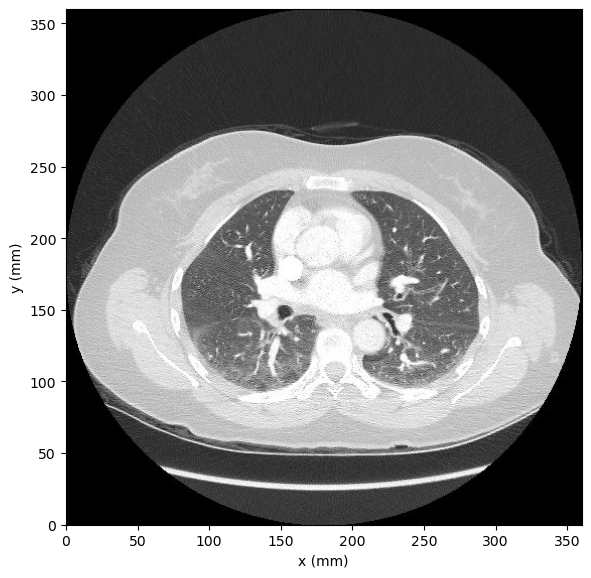
\includegraphics[width=0.9\linewidth]{Results/Axial_slice.png}
\caption{Axial slice at $z=118$.}
\label{fig:axial_slice}
\end{figure} 

\begin{figure}[h]
\centering
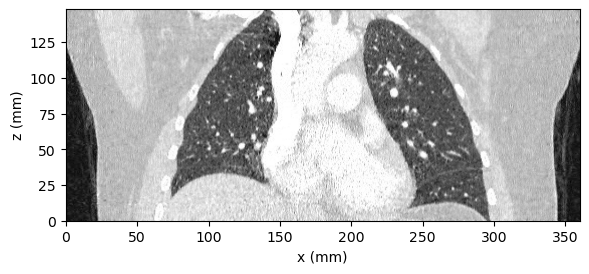
\includegraphics[width=0.9\linewidth]{Results/Coronal_slice.png}
\caption{Coronal slice at $y=256$.}
\label{fig:coronal_slice}
\end{figure} 

\begin{figure}[h]
\centering
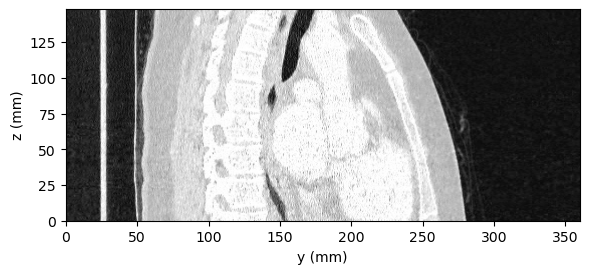
\includegraphics[width=0.9\linewidth]{Results/Sagittal_slice.png}
\caption{Sagittal slice at $x=256$.}
\label{fig:sagittal_slice}
\end{figure} 


\subsection{Salt and Pepper}

Figure \ref{fig:mean_median} shows the effects of mean and median filtering on the original axial slice using $3 \times 3$ and $5 \times 5$ kernels. The mean filter produced clear blurring, most pronounced with the $5 \times 5$ kernel, which obscured fine anatomical structures. The median filter preserved edges and structural boundaries more effectively, highlighting its suitability for noise reduction while maintaining image detail. However, increasing the kernel size also introduced some edge smoothing, making its output resemble that of the mean filter, though it still provided superior noise suppression and edge preservation.

\begin{figure}[h]
\centering
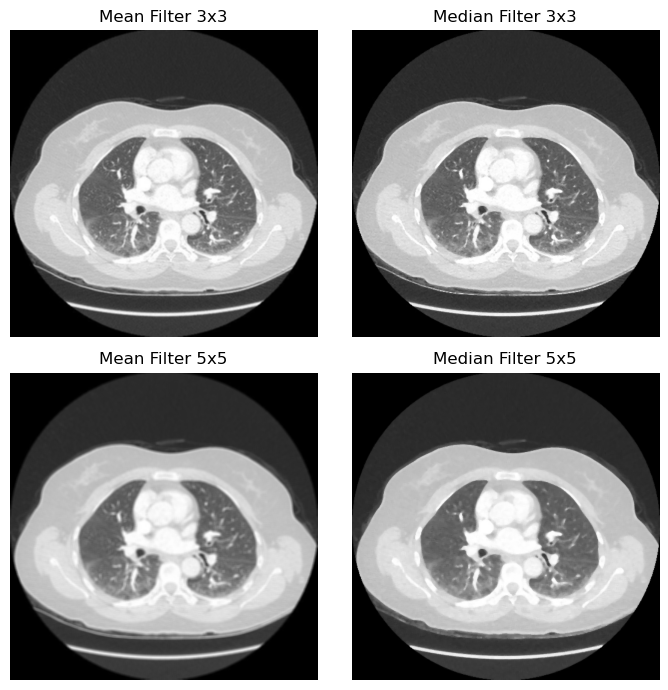
\includegraphics[width=0.9\linewidth]{Results/mean_median.png}
\caption{Mean and median filtered images.}
\label{fig:mean_median}
\end{figure}

Figure \ref{fig:snp} shows the performance of both filters after introducing salt-and-pepper noise at varying probabilities. The mean filter struggled to remove the noise, leaving substantial salt and pepper artifacts, particularly as the noise level increased. In contrast, the median filter removed most noise while preserving edges and anatomical detail, demonstrating strong robustness to this corruption. At the highest noise level ($p=0.1$), it still clearly outperformed the mean filter, although minor artifacts appeared in regions where local neighborhoods became heavily saturated with noisy pixels.

\begin{figure}[h]
\centering
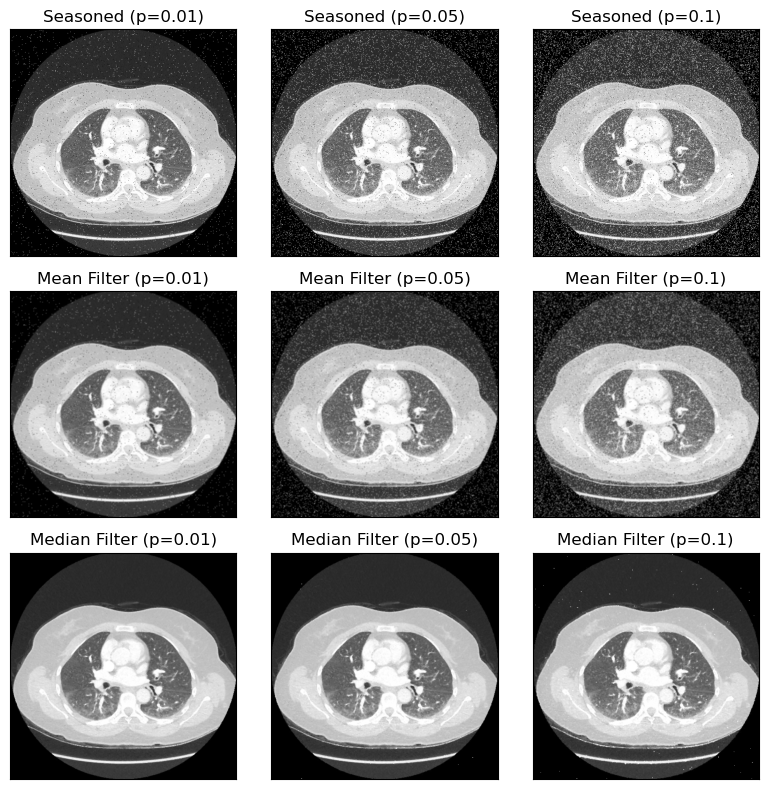
\includegraphics[width=0.9\linewidth]{Results/SNP.png}
\caption{Mean and median filtered images after artificial salt-and-pepper noise addition.}
\label{fig:snp}
\end{figure}

\subsection{Gaussian Noise and Blurring}

\subsubsection{2D Gaussian Noise \& Filtering}

Figure \ref{fig:2d_gauss} shows the effects of Gaussian noise addition and subsequent filtering on a 2D axial slice. The image was corrupted with Gaussian noise at $\sigma_{noise} = 10$ and $\sigma_{noise} = 20$, producing moderate grain in the former and substantially stronger degradation in the latter. Gaussian filtering was then applied with $\sigma_{filter} = 0.1$ and $\sigma_{filter} = 1.0$.

Noise addition degraded image quality as expected, with higher $\sigma_{noise}$ producing larger deviations from the underlying anatomical signal. Gaussian filtering improved the signal-to-noise ratio in both cases, but performance depended strongly on the match between noise level and filter width. For $\sigma_{noise} = 10$, a small filter ($\sigma_{filter} = 0.1$) reduced grain while largely preserving structural detail. For $\sigma_{noise} = 20$, stronger smoothing ($\sigma_{filter} = 1.0$) was required to suppress noise effectively.

This behavior reflects the inherent trade-off of Gaussian filtering. Increasing $\sigma_{filter}$ expands the spatial averaging neighborhood, improving noise suppression but attenuating high-frequency anatomical features. The heavily corrupted image ($\sigma_{noise} = 20$) required a larger filter, which reduced noise but produced noticeable blurring relative to the lightly filtered $\sigma_{noise} = 10$ case. Conversely, a small filter ($\sigma_{filter} = 0.1$) was insufficient for the noisier image, leaving visible grain, while a large filter ($\sigma_{filter} = 1.0$) applied to the less noisy image introduced unnecessary smoothing with minimal additional denoising benefit. These results emphasize that Gaussian filter parameters must be tuned to the noise level to balance denoising and structural preservation.

\begin{figure}[h]
\centering
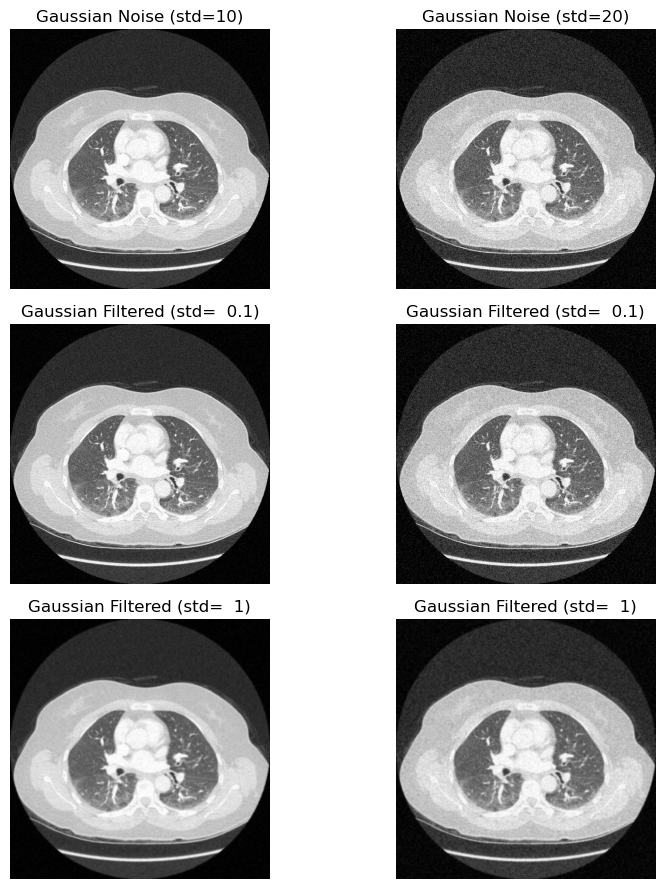
\includegraphics[width=0.9\linewidth]{Results/2d_gauss.png}
\caption{Gaussian-filtered axial slices for varying noise and filter standard deviations.}
\label{fig:2d_gauss}
\end{figure}

\subsubsection{3D Gaussian Blurring}

The 3D Gaussian blurring model was applied to the reconstructed volume, and representative slices were extracted from the axial, coronal, and sagittal mid-planes. Figures \ref{fig:3d_gauss_axial}--\ref{fig:3d_gauss_sagittal} show the resulting images.

Blurring is evident across all orientations, with reduced edge sharpness and attenuation of fine structures. The anisotropic parameters ($\delta x = \delta y = 2$ mm, $\delta z = 1$ mm) produce direction-dependent smoothing, though this is not visible via mere inspection. 

\begin{figure}[h]
\centering
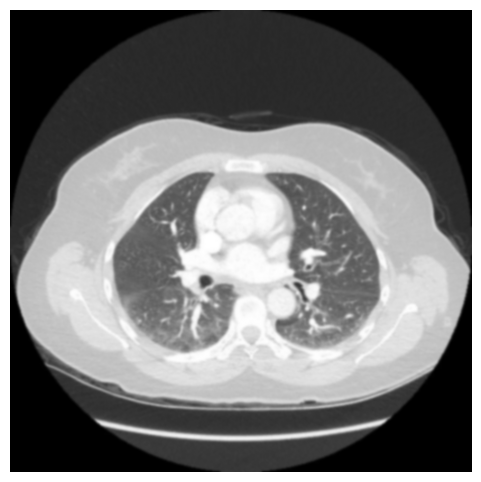
\includegraphics[width=0.9\linewidth]{Results/axial_3d_gauss.png}
\caption{Axial slice with 3D Gaussian blurring applied ($\delta x = 2$ mm, $\delta y = 2$ mm).}
\label{fig:3d_gauss_axial}
\end{figure}

\begin{figure}[h]
\centering
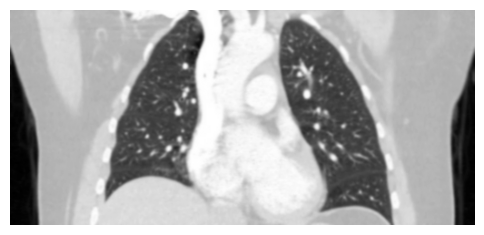
\includegraphics[width=0.9\linewidth]{Results/coronal_3d_gauss.png}
\caption{Coronal slice with 3D Gaussian blurring applied ($\delta x = 2$ mm, $\delta z = 1$ mm).}
\label{fig:3d_gauss_coronal}
\end{figure}

\begin{figure}[h]
\centering
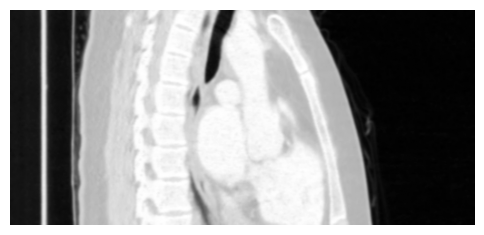
\includegraphics[width=0.9\linewidth]{Results/sagittal_3d_gauss.png}
\caption{Sagittal slice with 3D Gaussian blurring applied ($\delta y = 2$ mm, $\delta z = 1$ mm).}
\label{fig:3d_gauss_sagittal}
\end{figure}

\subsection{Foramina}

Figure \ref{fig:foramina} shows the results of Canny edge detection applied to the foramina region under varying preprocessing conditions, along with the raw coronal slice for reference.

\begin{figure*}[t]
\centering
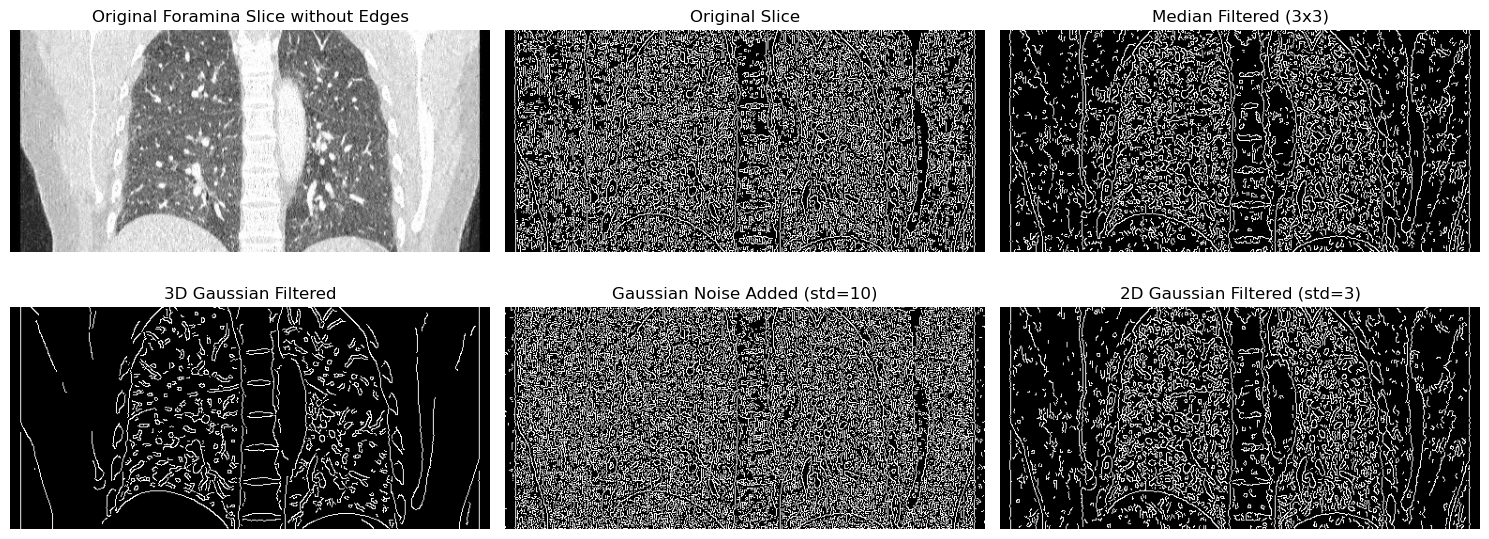
\includegraphics[width=0.9\linewidth]{Results/foramina.png}
\caption{Canny edge detection applied to the foramina region under varying preprocessing conditions.}
\label{fig:foramina}
\end{figure*}

Empirically, we can see that the edges of the foramina have low gradient magnitude (adjacent pixel intensities differ only slightly). Thus, the Canny edge detector's lower and higher thresholds were set to $50$ and $75$, respectively, to capture these subtle transitions. 

After Canny edge detection, the raw coronal slice and the Gaussian-noise-corrupted slice both produced highly fragmented edge maps, with no interpretable data. Raising the thresholds improved the results for detecting other anatomical edges, but completely eliminated the foramina edges, which were already weak in the original image.

The median filtered and 2D Gaussian filtered slices produced slightly more coherent edge maps, where the foramina are visible. However, they are still filled with spurious edges, so the foramina are quite difficult to distinguish from the noise.

The 3D Gaussian-blurred slice produced the most coherent edge map, where the foramina are clearly visible and distinguishable from other anatomical structures. The edges are smoother and more continuous, with fewer spurious detections. This is likely because the 3D Gaussian blurring simulates realistic system-level blur, which suppresses high-frequency noise while preserving broader anatomical boundaries.

Overall, the results illustrate a trade-off between noise suppression and edge fidelity, particularly for subtle features like the foramina. If we were to apply this edge detection to higher-contrast edges, it is likely that the median and 2D Gaussian filters would perform better, as they would preserve sharper transitions. However, for low-contrast features, the 3D Gaussian blurring appears to provide the best balance of noise reduction and edge preservation, enabling more reliable detection of subtle anatomical structures.

To explore the effect of edge detection on a higher-contrast edge, we applied Canny to an axial slice subject to the same preprocessing conditions, which is displayed in Figure \ref{fig:axial_canny}. For this process, the low and high Canny thresholds were set to $100$ and $200$, respectively. The edges of the lung fields and thoracic region are much stronger in this orientation, and thus the Canny edge detector was able to produce a more coherent edge map with fewer spurious detections. The noise-degraded image was uninterpretable, as expected, though notably less so than the foramina slice. Importantly, the median and 2D Gaussian filtered slices produced more coherent edge maps than the noisy foramina case, though the 3D Gaussian filtered slice still produced the most coherent results. This highlights the importance of both acquisition orientation and preprocessing in reliable edge extraction, particularly for low-contrast features like the foramina. 

\begin{figure*}[t]
\centering
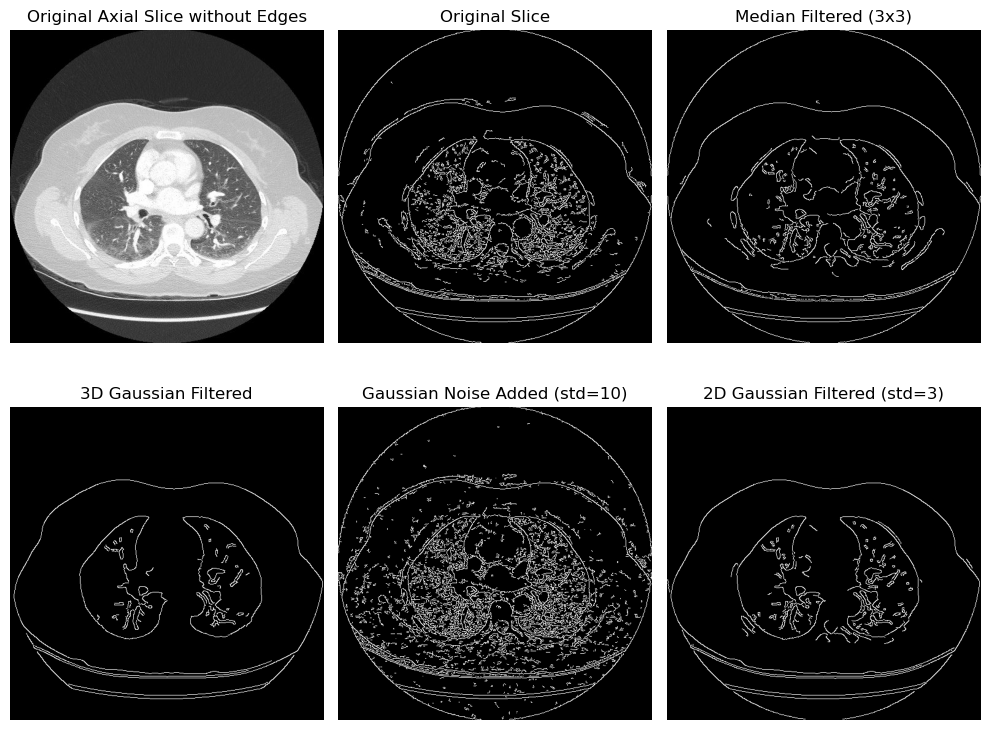
\includegraphics[width=0.9\linewidth]{Results/axial_canny.png}
\caption{Canny edge detection applied to an axial slice under varying preprocessing conditions.}
\label{fig:axial_canny}
\end{figure*}


\section{Conclusion}
The reconstructed CT volume enabled visualization across anatomical planes. While conventional filtering methods (mean, median, Gaussian) provided noise reduction, they also introduced the need for case-by-case parameter tuning (whether in kernel size or standard deviation). Edge detection performance depended strongly on preprocessing and feature contrast, with 3D Gaussian filtering offering the most coherent results for low-contrast structures such as foramina. Overall, the study emphasizes that appropriate modeling of noise and preprocessing is essential for preserving anatomical information and enabling reliable feature extraction in medical imaging workflows.


% --- Bibliography ---
\printbibliography

\end{document}